\documentclass[a4paper,11pt]{article}

% Kodovani (cestiny) v dokumentu: utf-8
%\usepackage[cp1250]{inputenc}	% Omezena stredoevropska kodova stranka, pouze MSW.
\usepackage[utf8]{inputenc}	% Doporucujeme pouzivat UTF-8 (unicode).

\usepackage[margin=2cm]{geometry}
\newtoks\jmenopraktika \newtoks\jmeno \newtoks\datum
\newtoks\obor \newtoks\skupina \newtoks\rocnik \newtoks\semestr
\newtoks\cisloulohy \newtoks\jmenoulohy
\newtoks\tlak \newtoks\teplota \newtoks\vlhkost

\jmenopraktika={Fyzikální praktikum 1}
\jmeno={Lukáš Lejdar}
\datum={7. května 2024}
\obor={F}
\skupina={Út 16:00}

\cisloulohy={6}
\jmenoulohy={Tepelné vlastnosti kapalin – elektrický kalorimetr}

\tlak={101{,}35}
\teplota={21,1}
\vlhkost={47,7}


%%%%%%%%%%% Uzitecne balicky:
\usepackage[czech]{babel}
\addto\captionsczech{\renewcommand{\figurename}{Graf}}

\usepackage{graphicx}
\usepackage{amsmath}
\usepackage{xspace}
\usepackage{url}
\usepackage{indentfirst}
\usepackage{wrapfig}
\usepackage{xcolor}

%%%%%% Zamezeni parchantu:
\widowpenalty 10000 \clubpenalty 10000 \displaywidowpenalty 10000
%%%%%% Parametry pro moznost vsazeni vetsiho poctu obrazku na stranku
\setcounter{topnumber}{3}	  % max. pocet floatu nahore (specifikace t)
\setcounter{bottomnumber}{3}	  % max. pocet floatu dole (specifikace b)
\setcounter{totalnumber}{6}	  % max. pocet floatu na strance celkem
\renewcommand\topfraction{0.9}	  % max podil stranky pro floaty nahore
\renewcommand\bottomfraction{0.9} % max podil stranky pro floaty dole
\renewcommand\textfraction{0.1}	  % min podil stranky, ktery musi obsahovat text
\intextsep=8mm \textfloatsep=8mm  %\intextsep pro ulozeni [h] floatu a \textfloatsep pro [b] or [t]

% Tecky za cisly sekci:
\renewcommand{\thesection}{\arabic{section}.}
\renewcommand{\thesubsection}{\thesection\arabic{subsection}.}
% Jednopismenna mezera mezi cislem a nazvem kapitoly:
\makeatletter \def\@seccntformat#1{\csname the#1\endcsname\hspace{1ex}} \makeatother
%
\newcommand{\vsn}[4]{\ensuremath{#1 =} #2(#3)\,#4}
\newcommand{\vrn}[6]{\ensuremath{#1 =} (#2 $\pm$ #3)\,#4 ($p=$ #5\,\%, $\nu=$ #6)}


%%%%%%%%%%%%%%%%%%%%%%%%%%%%%%%%%%%%%%%%%%%%%%%%%%%%%%%%%%%%%%%%%%%%%%%%%%%%%%%
% Zacatek dokumentu
%%%%%%%%%%%%%%%%%%%%%%%%%%%%%%%%%%%%%%%%%%%%%%%%%%%%%%%%%%%%%%%%%%%%%%%%%%%%%%%

\begin{document}

\thispagestyle{empty}

{
\begin{center}
\sf 
{\Large Ústav fyziky a technologií plazmatu Přírodovědecké fakulty Masarykovy univerzity} \\
\bigskip
{\huge \bfseries FYZIKÁLNÍ PRAKTIKUM} \\
\bigskip
{\Large \the\jmenopraktika}
\end{center}

\bigskip

\sf
\noindent
\setlength{\arrayrulewidth}{1pt}
\begin{tabular*}{\textwidth}{@{\extracolsep{\fill}} l l}
\large {\bfseries Zpracoval:}  \the\jmeno & \large  {\bfseries Naměřeno:} \the\datum\\[2mm]
\large  {\bfseries Obor:} \the\obor  \hspace{40mm}  {\bfseries Skupina:} \the\skupina %
&\large {\bfseries Testováno:}\\
\\
\hline
\end{tabular*}
}

\bigskip

{
\sf
\noindent \begin{tabular}{p{4cm} p{0.6\textwidth}}
\Large  Úloha č. {\bfseries \the\cisloulohy:} \par
\smallskip
$T=\the\teplota$~$^\circ$C \par
$p=\the\tlak$~kPa \par
$\varphi=\the\vlhkost$~\%
&\Large \bfseries \the\jmenoulohy  \\[2mm]
\end{tabular}
}

\vskip1cm

\section{Úvod}

Elektrický kalorimetr je zařízení, které umožňuje měřit tepelnou kapacitu látky v něm. V úloze si jeden kalorimetr poskládám a pokusím se ho zkalibrovat. Zároveň bych měl být schopný dopočítat měrnou tepelnou kapacitu kalibrační kapaliny. V úloze použiju kohoutkovou vodu.

\section{Teorie}

Fyzicky je elektrický kalorimetr tepelně izolovaná nádoba s teploměrem, míchačkou a elektrickou topnou spirálou o výkonu $UI$. Dokud v něm probíhají tepelné změny pomalu, můžu pro něj vyjádřit 1. termodynamický zákon

\begin{align}
  dE &= UId\tau \\ 
     &= (mc + K)dt,
\end{align}

\noindent
kde K je kapacita kalorimetru, $\tau$ je čas, m hmotnosti látky a c její měrná tepelná kapacita. Pro reálné kalorimetry je ale potřeba uvažovat i ztráty do okolí $dQ_{\text{s}}$. Předpokládejme, že jsou podle Newtonova zákona přímo úměrné rozdílu teplot oproti teplotě okolí $t_0$

\begin{align}
  dQ_{\text{s}} &= \beta(t - t_0)d\tau \\
  UId\tau &= (mc + K)dt + dQ_{\text{s}}
\end{align}

\noindent
přičemž veličina $\beta$ je takto definovaný koeficient chladnutí. Je víc způsobů jak kalorimetr použít, vždycky ale bude prvně potřeba znát kapacitu K a koeficient chladnutí $\beta$.

\subsection{Měření koeficientu chladnutí kalorimetru $\beta$}
Uvažujme řešení rovnice (2), kde v čase $\tau=0$ je teplota kalorimetru rovná teplotě okolí (t = $t_0$) a látku uvnitř ohřívá nenulový výkon spirály. Dosazením dostávám

\begin{align}
  UI &= (mc + K) \frac{dt}{d\tau}(0).
\end{align}

\noindent
Zrealizuju popsaný experiment, změřím rychlost růstu teploty na začátku a dozvím se celkovou tepelnou kapacitu $(mc + K)$. Pokud nechám kapalinu dál ohřívat, bude růst rozdíl teplot $(t - t_0)$ a nakonec se ztráty do okolí vyrovnají příkonu $UI$. Je to moment v čase $\tau_{\text{f}}$ , kdy $dt$ = 0.

\begin{equation}
UI = \beta (t_{\text{f}} - t_0)
\end{equation}

\noindent
Mohl, bych opravdu počkat než se teplota ustálí, ale to by přesahovalo dobu trvání praktika. Místo toho vyřeším analyticky rovnici (2) pro popsané počáteční podmínky

\begin{equation}
t = t_0 + \frac{UI}{\beta} \left(1 - e^{-\frac{\beta}{mc + K}\tau}\right)
\end{equation}

\noindent
a koeficient chladnutí $\beta$ určím z fitu exponenciely, kde už znám $(mc + K)$. Tento výraz ještě přepíšu pomocí redukované kapacity kalorimetru $\kappa = \frac{K}{c}$ jako

\begin{align}
 mc + K &= c(m + \kappa),
\end{align}

\noindent
kde k dopočítání měrné tepelné kapacity ještě potřebuji změřit $\kappa$.


\subsection{Měření kapacity kalorimetru K}

Do kalorimetru naplněného kapalinou o počáteční teplotě $t_1$ a hmotnosti $m_1$ přidám tu samou kapalinu o teplotě $t_2 > t_1$ a hmotnosti $m_2$. Platí kalorimetrická rovnice

\begin{equation}
(m_1c + K)(t-t_1) = m_2c(t_2-t)
\end{equation}

\noindent
do které dosadím redukovanou kapacitu 

\begin{align}
  c(m_1 + \kappa)(t-t_1) &= m_2c(t_2-t) \\
  (m_1 + \kappa)(t-t_1) &= m_2(t_2-t)
\end{align}

\noindent
a měrné tepelné kapacity se zkrátí. Vyjádřím $\kappa$

\begin{align}
  \kappa &= m_2 \frac{t_2 - t}{t - t_1} - m_1
\end{align}

\noindent
odkud spolu se vztahem (8) můžu dopočítat měrnou tepelnou kapacitu c i kapacitu kalorimetru K, pokud jsem použil tu stejnou kapalinu.

\section{Postup měření}

Kalorimetr normálně chceme mít s co nejmenšími ztrátami do okolí, abychom ho při běžném používání mohli považovat za úplně izolovaný. Při konstrukci toho mého se budu v zájmu kratšího měření snažit o opak. Na magnetickou míchačku položím větší kádinku, kterou můžu přiklopit víkem s visutou topnou spirálou a otvory pro teploměry. Nádoba je uzavřená, takže výměna tepla ven z kádinky bude probíhat pouze vedením a tím splňuje podmínky kalorimetru. Jako kalibrační kapalinu použiju vodu z kohoutku.

\section{Výsledky měření}

\subsection{Měření koeficientu chladnutí kalorimetru $\beta$}

Naplnil jsem kalorimetr vodou o hmotnosti $m_{\beta} = (349.50 \pm 0.04)$ g a počkal než se teplota vyrovná s teplotou okolí. Potom jsem zapojil topnou spirálu ke zdroji o příkonu 20 W a měřil teplotu v kádince. Naměřené hodnoty jsou uvedené v grafu 1. a fit je rovnicí (7).

\begin{figure}[htpb]
  \centering
  % GNUPLOT: LaTeX picture with Postscript
\begingroup
  \makeatletter
  \providecommand\color[2][]{%
    \GenericError{(gnuplot) \space\space\space\@spaces}{%
      Package color not loaded in conjunction with
      terminal option `colourtext'%
    }{See the gnuplot documentation for explanation.%
    }{Either use 'blacktext' in gnuplot or load the package
      color.sty in LaTeX.}%
    \renewcommand\color[2][]{}%
  }%
  \providecommand\includegraphics[2][]{%
    \GenericError{(gnuplot) \space\space\space\@spaces}{%
      Package graphicx or graphics not loaded%
    }{See the gnuplot documentation for explanation.%
    }{The gnuplot epslatex terminal needs graphicx.sty or graphics.sty.}%
    \renewcommand\includegraphics[2][]{}%
  }%
  \providecommand\rotatebox[2]{#2}%
  \@ifundefined{ifGPcolor}{%
    \newif\ifGPcolor
    \GPcolorfalse
  }{}%
  \@ifundefined{ifGPblacktext}{%
    \newif\ifGPblacktext
    \GPblacktexttrue
  }{}%
  % define a \g@addto@macro without @ in the name:
  \let\gplgaddtomacro\g@addto@macro
  % define empty templates for all commands taking text:
  \gdef\gplbacktext{}%
  \gdef\gplfronttext{}%
  \makeatother
  \ifGPblacktext
    % no textcolor at all
    \def\colorrgb#1{}%
    \def\colorgray#1{}%
  \else
    % gray or color?
    \ifGPcolor
      \def\colorrgb#1{\color[rgb]{#1}}%
      \def\colorgray#1{\color[gray]{#1}}%
      \expandafter\def\csname LTw\endcsname{\color{white}}%
      \expandafter\def\csname LTb\endcsname{\color{black}}%
      \expandafter\def\csname LTa\endcsname{\color{black}}%
      \expandafter\def\csname LT0\endcsname{\color[rgb]{1,0,0}}%
      \expandafter\def\csname LT1\endcsname{\color[rgb]{0,1,0}}%
      \expandafter\def\csname LT2\endcsname{\color[rgb]{0,0,1}}%
      \expandafter\def\csname LT3\endcsname{\color[rgb]{1,0,1}}%
      \expandafter\def\csname LT4\endcsname{\color[rgb]{0,1,1}}%
      \expandafter\def\csname LT5\endcsname{\color[rgb]{1,1,0}}%
      \expandafter\def\csname LT6\endcsname{\color[rgb]{0,0,0}}%
      \expandafter\def\csname LT7\endcsname{\color[rgb]{1,0.3,0}}%
      \expandafter\def\csname LT8\endcsname{\color[rgb]{0.5,0.5,0.5}}%
    \else
      % gray
      \def\colorrgb#1{\color{black}}%
      \def\colorgray#1{\color[gray]{#1}}%
      \expandafter\def\csname LTw\endcsname{\color{white}}%
      \expandafter\def\csname LTb\endcsname{\color{black}}%
      \expandafter\def\csname LTa\endcsname{\color{black}}%
      \expandafter\def\csname LT0\endcsname{\color{black}}%
      \expandafter\def\csname LT1\endcsname{\color{black}}%
      \expandafter\def\csname LT2\endcsname{\color{black}}%
      \expandafter\def\csname LT3\endcsname{\color{black}}%
      \expandafter\def\csname LT4\endcsname{\color{black}}%
      \expandafter\def\csname LT5\endcsname{\color{black}}%
      \expandafter\def\csname LT6\endcsname{\color{black}}%
      \expandafter\def\csname LT7\endcsname{\color{black}}%
      \expandafter\def\csname LT8\endcsname{\color{black}}%
    \fi
  \fi
    \setlength{\unitlength}{0.0500bp}%
    \ifx\gptboxheight\undefined%
      \newlength{\gptboxheight}%
      \newlength{\gptboxwidth}%
      \newsavebox{\gptboxtext}%
    \fi%
    \setlength{\fboxrule}{0.5pt}%
    \setlength{\fboxsep}{1pt}%
    \definecolor{tbcol}{rgb}{1,1,1}%
\begin{picture}(7920.00,3614.00)%
    \gplgaddtomacro\gplbacktext{%
      \csname LTb\endcsname%%
      \put(682,36){\makebox(0,0)[r]{\strut{}$20$}}%
      \put(682,386){\makebox(0,0)[r]{\strut{}$25$}}%
      \put(682,735){\makebox(0,0)[r]{\strut{}$30$}}%
      \put(682,1085){\makebox(0,0)[r]{\strut{}$35$}}%
      \put(682,1435){\makebox(0,0)[r]{\strut{}$40$}}%
      \put(682,1784){\makebox(0,0)[r]{\strut{}$45$}}%
      \put(682,2134){\makebox(0,0)[r]{\strut{}$50$}}%
      \put(682,2484){\makebox(0,0)[r]{\strut{}$55$}}%
      \put(682,2834){\makebox(0,0)[r]{\strut{}$60$}}%
      \put(682,3183){\makebox(0,0)[r]{\strut{}$65$}}%
      \put(814,-184){\makebox(0,0){\strut{}$0$}}%
      \put(1485,-184){\makebox(0,0){\strut{}$500$}}%
      \put(2156,-184){\makebox(0,0){\strut{}$1000$}}%
      \put(2827,-184){\makebox(0,0){\strut{}$1500$}}%
      \put(3498,-184){\makebox(0,0){\strut{}$2000$}}%
      \put(4169,-184){\makebox(0,0){\strut{}$2500$}}%
      \put(4839,-184){\makebox(0,0){\strut{}$3000$}}%
      \put(5510,-184){\makebox(0,0){\strut{}$3500$}}%
      \put(6181,-184){\makebox(0,0){\strut{}$4000$}}%
      \put(6852,-184){\makebox(0,0){\strut{}$4500$}}%
      \put(7523,-184){\makebox(0,0){\strut{}$5000$}}%
      \put(975,3183){\makebox(0,0)[l]{\strut{}$\beta = (0.4881 \pm 0.0001)$ WK$^{-1}$}}%
      \put(975,2834){\makebox(0,0)[l]{\strut{}$K_{\beta} = (1585 \pm 5)$ JK$^{-1}$}}%
    }%
    \gplgaddtomacro\gplfronttext{%
      \csname LTb\endcsname%%
      \put(6536,3220){\makebox(0,0)[r]{\strut{}$t(\tau)$}}%
      \csname LTb\endcsname%%
      \put(6536,3000){\makebox(0,0)[r]{\strut{}$t_0$}}%
      \csname LTb\endcsname%%
      \put(6536,2780){\makebox(0,0)[r]{\strut{}fit}}%
      \csname LTb\endcsname%%
      \put(209,1714){\rotatebox{-270.00}{\makebox(0,0){\strut{}T ($^{\circ}$C)}}}%
      \put(4168,-514){\makebox(0,0){\strut{}t (s)}}%
    }%
    \gplbacktext
    \put(0,0){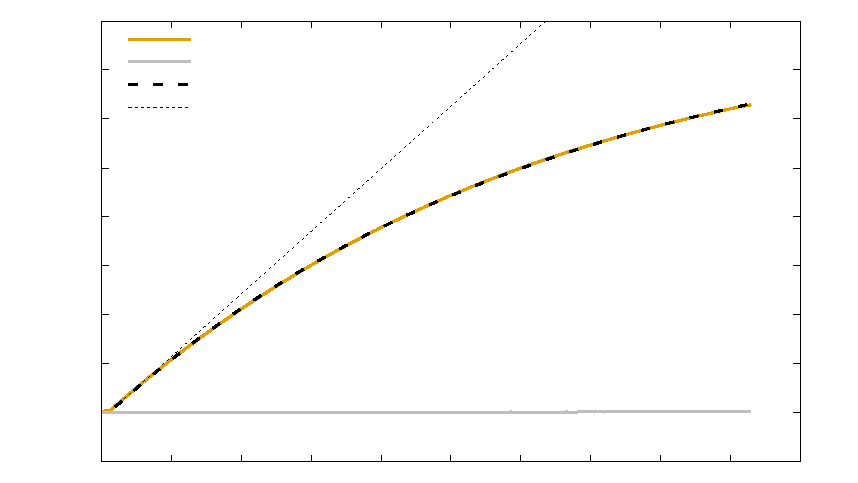
\includegraphics[width={396.00bp},height={180.70bp}]{ohrev_kalorimetru}}%
    \gplfronttext
  \end{picture}%
\endgroup

  \caption{Závislost teploty v kalorimetru na čase}
  \vspace{-30pt}
\end{figure}


\begin{align*}
  \beta &= (0.4881 \pm 0.0001) WK^{-1} \\
  mc + K &= (1585 \pm 5) JK^{-1}
\end{align*}

\vspace{5pt}

\subsection{Měření kapacity kalorimetru K}

Připravil jsem kádinku s vodou o teplotě $t_2$ = $ (41.90 \pm 0.05)\ ^{\circ}C$ a hmotnosti $m_2 = (236.6 \pm 0.2)$ g a kalorimetr naplnil vodou o teplotě $t_1 = (24.1 \pm 0.05)\ ^{\circ}C$ a hmotnosti $m_1 = (429.0 \pm 0.2)$ g. Po přelití teplejší vody do kalorimetru se teplota ustálila na $t=(30.10 \pm 0.05)\ ^{\circ}C$. Ze vztahu (12) vypočítám redukovanou kapacitu $\kappa$ a ze vztahu (8) měrnou tepelnou kapacitu vody c a kapacitu kalorimetru K.


\begin{align*}
  \kappa &= (0.036 \pm 0.007)\ kg \\
  K &= (149 \pm 30) \text{ JK}^{-1} \\
  c_{\text{v}} &=  (4110 \pm 80) \text{ JK}^{-1}\text{kg}^{-1}
\end{align*}

\section{Závěr}

Postavil jsem kalorimetr z kádinky a změřil jeho kapacitu $K = (149 \pm 30)$ JK$^{-1}$ a koeficient chladnutí $\beta = (0.4881 \pm 0.0001)$ WK$^{-1}$. Navíc jsem změřil i měrnou tepelnou kapacitu vody $c_{\text{v}} = (4110 \pm 80)$ JK$^{-1}$kg$^{-1}$. Tabulky udávají hodnotu 4180 JK$^{-1}$kg$^{-1}$. Největším zdrojem nejistoty jsou nejisoty teplot $t_1$, $t_2$ a $t$. Ve vztahu (12) se totiž odčítají dvě velmi podobné hodnoty 

\begin{align*}
  m_2 \frac{t_2 - t}{t - t_1} &= (0.465 \pm 0.007) g \\
  m_1 &= (0.429 \pm 0.00002) g
\end{align*}

\noindent
a velká část přesnosti měření se tak ztratí.


\end{document}
